\subsection{bpmorbit/vm.c File Reference}
\label{vm_8c}\index{bpmorbit/vm.c@{bpmorbit/vm.c}}


\subsubsection{Detailed Description}


Definition in file {\bf vm.c}.

{\tt \#include $<$bpm/bpm\_\-orbit.h$>$}\par
{\tt \#include $<$stdlib.h$>$}\par
{\tt \#include $<$stdio.h$>$}\par
{\tt \#include $<$math.h$>$}\par


Include dependency graph for vm.c:\nopagebreak
\begin{figure}[H]
\begin{center}
\leavevmode
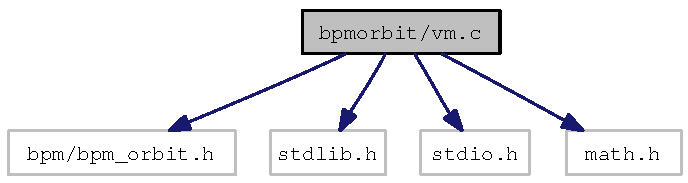
\includegraphics[width=183pt]{vm_8c__incl}
\end{center}
\end{figure}
\subsubsection*{Functions}
\begin{CompactItemize}
\item 
void {\bf v\_\-copy} (struct {\bf v3} $\ast$v1, struct {\bf v3} $\ast$v2)
\item 
double {\bf v\_\-mag} (struct {\bf v3} $\ast$v1)
\item 
void {\bf v\_\-scale} (struct {\bf v3} $\ast$v1, double dscale)
\item 
void {\bf v\_\-norm} (struct {\bf v3} $\ast$v1)
\item 
void {\bf v\_\-matmult} (struct {\bf m33} $\ast$m1, struct {\bf v3} $\ast$v1)
\item 
void {\bf v\_\-add} (struct {\bf v3} $\ast$v1, struct {\bf v3} $\ast$v2)
\item 
void {\bf v\_\-sub} (struct {\bf v3} $\ast$v1, struct {\bf v3} $\ast$v2)
\item 
double {\bf v\_\-dot} (struct {\bf v3} $\ast$v1, struct {\bf v3} $\ast$v2)
\item 
void {\bf v\_\-cross} (struct {\bf v3} $\ast$v1, struct {\bf v3} $\ast$v2)
\item 
void {\bf v\_\-print} (struct {\bf v3} $\ast$v1)
\item 
void {\bf m\_\-rotmat} (struct {\bf m33} $\ast$m1, double alpha, double beta, double gamma)
\item 
void {\bf m\_\-matmult} (struct {\bf m33} $\ast$m, struct {\bf m33} $\ast$m1, struct {\bf m33} $\ast$m2)
\item 
void {\bf m\_\-matadd} (struct {\bf m33} $\ast$m1, struct {\bf m33} $\ast$m2)
\item 
void {\bf m\_\-print} (struct {\bf m33} $\ast$m1)
\end{CompactItemize}
